\documentclass{article}

\usepackage[left=3cm,right=3cm,top=4cm,bottom=3cm]{geometry}
\usepackage{graphicx}
\usepackage{float}
\usepackage{algorithm}
\usepackage{algpseudocode}

\title{\textbf{The MECA Block Cipher}}
\author{John Holly}
\date{\today}

\thispagestyle{plain}
\graphicspath{ {../img/key-schedule}{../img/metamorphic-engine} }

\begin{document}

\maketitle

\algblock{Input}{EndInput}
\algnotext{EndInput}
\algblock{Output}{EndOutput}
\algnotext{EndOutput}
\newcommand{\Desc}[2]{\State \makebox[2em][l]{#1}#2}

\begin{abstract}
  \centering
  \begin{minipage}{\dimexpr\paperwidth-10cm}
    TODO
  \end{minipage}
\end{abstract}

\bigskip

\section{Introduction}

MECA is a novel block cipher utilizing second-order cellular automata (MECA) and metamorphic engines in both encryption/decryption rounds and key scheduling.

The design of MECA began with inspiration from a handful of other well known ciphers: RC6\cite{RC6} for its small size and simplicity, speed, and elegant extensibility to different word sizes, rounds, and key length, Stone Cipher-192 (SC-192)\cite{SC-192} for its crypto logic unit (metamorphic engine, or CLU), and a variety of papers I've read on novel ciphers utilizing first-order elementary cellular automata.

The MECA cipher was designed to be simplistic and easily understood to those without a deep knowledge of mathematics and cryptography. The goals in mind were simplistic chaos that can be easily visualized, extensibility, efficiency in both hardware and software implementations, and exploitation of the reversibility of second-order cellular automata in place of traditional feistel networks.

\section{Details}

Similarly to RC5 and RC6, MECA is fully parameterized and can be specified as MECA-$w$/$r$/$b$ with the word size (registers) being $w$ bits, $r$ encryption rounds, and $b$ bytes in the encryption key. Metamorphic logic units and cellular automata (both first-order and second-order) are the primitive building blocks throughout the cipher. Much like feistel networks can be run in reverse with the same logic as forwards, MECAs can be run in reverse by simply swapping the pre-initial and initial states (the previous and current timesteps [state] of the cellular automata) the forward pass (encryption) converged to.

\subsection{Metamorphic Engines (CLUs)}

TODO: Will there be three metamorphic engines? One for the binop of combining key with plaintext.

There are two metamorphic engines in use, one using irreversible first-order CA rules as a one-way hashing function for the key-generating-key (unscheduled, the one of $b$ bytes specified as a parameter), and one used during encryption/decryption rounds selecting the second-order rules per round. The first-order engine selects from 3 class 4 elementary CA rules. The second-order engine selects from 7 cherry-picked rules that also display globally chaotic behavior\cite{MECA-Properties}.

\subsubsection{First-order CLU}

The first-order CLU selects a class 4 elementary CA rule based on the remainder ($mod$ 3) of the key-generating-key word at index $i$ of a specific iteration in the scheduling algorithm XORed with the current key schedule key at index $j$. The mappings are shown in table \ref{tab:table1} and the rules are shown evolved with random initial conditions in figures \ref{fig:figure1}, \ref{fig:figure2}, \ref{fig:figure3}.

\begin{table}[h!]
  \begin{center}
    \caption{First-order CLU mapping}
    \label{tab:table1}
    \begin{tabular}{l|c|r} % <-- Alignments: 1st column left, 2nd middle and 3rd right, with vertical lines in between
      \textbf{Remainder} & \textbf{Rule}\\
      \hline
      0 & 54\\
      1 & 110\\
      2 & 137\\
    \end{tabular}
  \end{center}
\end{table}

\begin{figure}[H]
  \begin{center}
    \begin{minipage}{0.48\textwidth}
      \caption{Rule 54}
      \label{fig:figure1}
      \centering
      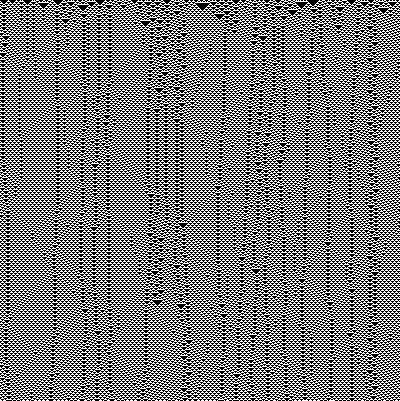
\includegraphics[scale=.5]{54.png}
    \end{minipage}
    \begin{minipage}{0.48\textwidth}
      \caption{Rule 110}
      \label{fig:figure2}
      \centering
      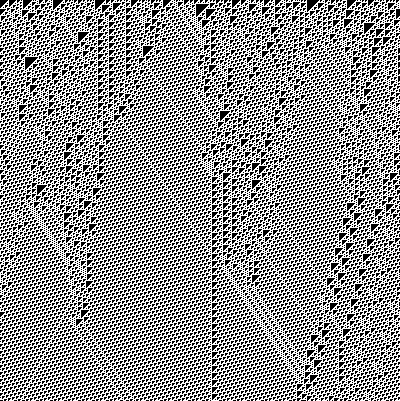
\includegraphics[scale=.5]{110.png}
    \end{minipage}
  \end{center}
\end{figure}
\begin{figure}[H]
  \begin{center}
    \begin{minipage}{0.48\textwidth}
      \caption{Rule 137}
      \label{fig:figure3}
      \centering
      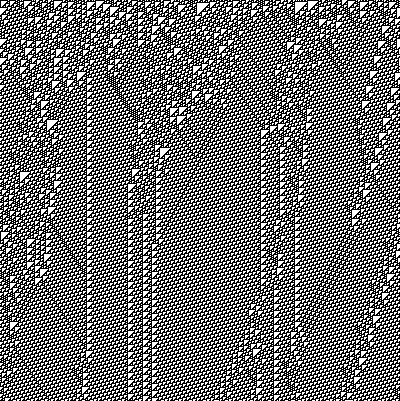
\includegraphics[scale=.5]{137.png}
    \end{minipage}
  \end{center}
\end{figure}

\subsubsection{Second-order CLU}

The second-order CLU selects a chaotic second-order rule based on the remainder ($mod$ 7) of the current state of the MECA (timestep $t$). The mappings are shown in table \ref{tab:table2}.

\begin{table}[h!]
  \begin{center}
    \caption{Second-order CLU mapping}
    \label{tab:table2}
    \begin{tabular}{l|c|r} % <-- Alignments: 1st column left, 2nd middle and 3rd right, with vertical lines in between
      \textbf{Remainder} & \textbf{Rule}\\
      \hline
      0 & 75\\
      1 & 86\\
      2 & 89\\
      3 & 149\\
      4 & 166\\
      5 & 173\\
      6 & 229\\
    \end{tabular}
  \end{center}
\end{table}

\begin{figure}[H]
  \begin{center}
    \begin{minipage}{0.48\textwidth}
      \caption{Rule 75}
      \label{fig:figure4}
      \centering
      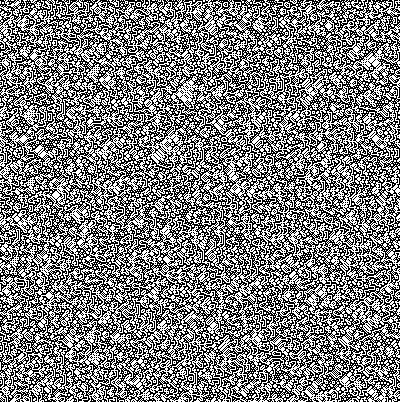
\includegraphics[scale=.5]{75.png}
    \end{minipage}
    \begin{minipage}{0.48\textwidth}
      \caption{Rule 86}
      \label{fig:figure5}
      \centering
      
\includegraphics[scale=.5]{86.png}
    \end{minipage}
    \begin{minipage}{0.48\textwidth}
      \caption{Rule 89}
      \label{fig:figure6}
      \centering
      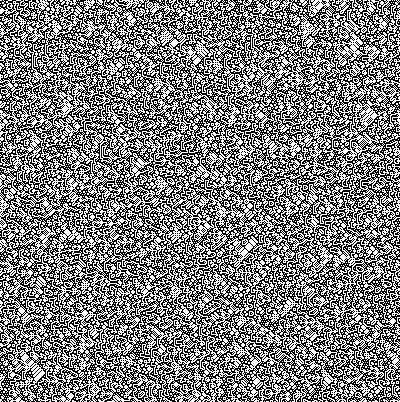
\includegraphics[scale=.5]{89.png}
    \end{minipage}
    \begin{minipage}{0.48\textwidth}
      \caption{Rule 149}
      \label{fig:figure7}
      \centering
      
\includegraphics[scale=.5]{149.png}
    \end{minipage}
  \end{center}
\end{figure}
\begin{figure}[H]
  \begin{center}
    \begin{minipage}{0.48\textwidth}
      \caption{Rule 166}
      \label{fig:figure8}
      \centering
      
\includegraphics[scale=.5]{166.png}
    \end{minipage}
    \begin{minipage}{0.48\textwidth}
      \caption{Rule 173}
      \label{fig:figure9}
      \centering
      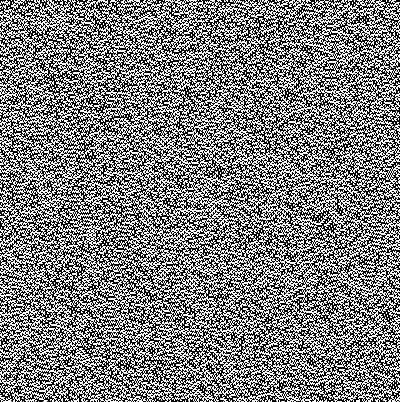
\includegraphics[scale=.5]{173.png}
    \end{minipage}
    \begin{minipage}{0.48\textwidth}
      \caption{Rule 229}
      \label{fig:figure10}
      \centering
      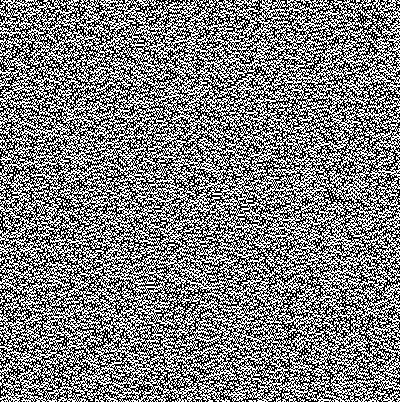
\includegraphics[scale=.5]{229.png}
    \end{minipage}
  \end{center}
\end{figure}

\subsection{Key Schedule}

The key schedule uses the same magic constants for initialization as RC6. Let $P$ be the binary expansion of $e-2$ and $Q$ is the binary expansion of $\varphi-1$, where $\varphi$ is the golden ratio. The metamorphic engine for CA rule selection is defined by the piecewise function below.

$$
  m(x) = \cases{ 54  & $x$ $mod$ $3 = 0$ \cr
                 110 & $x$ $mod$ $3 = 1$ \cr
                 137 & $x$ $mod$ $3 = 2$ }
$$

The function for the outcome of a single timestep with a given rule is defined by the function below. Let $m(x)$ be the desired rule and $c(S_i, m(x))$ is the execution of the elementary CA, where $S_i$ is the resulting round key (for a given iteration).

$$
 S_i = c(S_i, m(x)) 
$$

\begin{algorithm}[H]
  \begin{algorithmic}
    \caption{Key schedule for MECA-$w$/$r$/$b$}\label{alg:schedule}
    \Input
      \Desc{L}{$b$ byte key preloaded into $c$-word array}
      \Desc{r}{number of rounds}
    \EndInput
    \Output
      \Desc{$S$}{$w$-bit round keys $S[0, ..., 2r - 1]$}
    \EndOutput
    \State $S[0] = P$
    \For{$i \gets 1$ to $2r-1$} 
      \State {$S[i]$ $\gets$ {$S[i-1] + Q$}}
    \EndFor
    \State $j \gets 0$
    \State $i \gets 0$
    \For{$s \gets 0$ to max(c, $2r$)}
      \State $S[i] \gets c(S[i], m(L[j] \oplus S[i]))$ 
      \State $i \gets i+1$ $mod$ $2r-1$
      \State $j \gets j+1$ $mod$ $c-1$
    \EndFor
  \end{algorithmic}
\end{algorithm}

\subsection{Encryption}

\subsection{Decryption}

\section{Key Schedule}

\section{Encryption and Decryption}

\section{Performance}

\section{Implementation Issues}

\section{Design and Motivation}

\section{Security}

\section{Flexibility and Future Direction}

\section{Conclusions}

\section{Acknowledgements}

\begin{thebibliography}{unsrt}
  \bibitem{RC6}
  Ronald L. Rivest, M.J.B. Robshaw, R. Sidney, and Y.L. Yin, \emph{The RC6\texttrademark Block Cipher} (First Advanced Encryption Standard (AES) Conference, USA, 1998).
  \bibitem{SC-192}
  Magdy Saeb, \emph{The Stone Cipher-192 (SC-192): A Metamorphic Cipher} (IJCNS) International Journal of Computer and Network Security, 2009
  \bibitem{MECA-Properties}
  A. H. Encinas, A. M. d. Rey, J. L. P. Iglesias, G. R. Sánchez and A. Q. Dios, \emph{Cryptographic Properties of Second-Order Memory Elementary Cellular Automata} 2008 Third International Conference on Availability, Reliability and Security, 2008, pp. 741-745, doi: 10.1109/ARES.2008.114.
\end{thebibliography}
\end{document}